\documentclass[11pt, twoside]{report} % Tipo di documento

%------------------------------------------------------------------------------

% Pacchietti importati
\usepackage{
    amsmath, amsthm, amssymb, calrsfs, wasysym, bbm, color, graphics,
    geometry, fancyhdr, xcolor, graphicx, caption, subcaption, pifont, hyperref,
    commath, wrapfig, latexsym, shadethm, verbatim, listings
}
%------------------------------------------------------------------------------

% Font
\usepackage[utf8]{inputenc}
\usepackage{cmbright}
\usepackage[OT1]{fontenc}
\usepackage[italian]{babel}
%------------------------------------------------------------------------------

% Impaginazione
\pagestyle{fancy}
\setlength{\headheight}{15pt}
\renewcommand{\headrulewidth}{0.4pt}
\geometry{a4paper,width=150mm,top=25mm,bottom=25mm,bindingoffset=6mm}  

\fancyhead[LE,RO]{}

\renewcommand{\chaptermark}[1]{\markboth{\chaptername\ \thechapter.\ #1}{}}
%------------------------------------------------------------------------------

% Simboli matematici
\newcommand{\R}{\mathbb{R}}
\newcommand{\C}{\mathbb{C}}
\newcommand{\Z}{\mathbb{Z}}
\newcommand{\N}{\mathbb{N}}
\newcommand{\Q}{\mathbb{Q}}
\newcommand{\A}{\mathbb{A}}

%
\newtheorem{definition}{Definizione}[chapter]
\newtheorem{theorem}{Teorema}[chapter]
\newtheorem{property}{Proprietà}[chapter]

%------------------------------------------------------------------------------

% Blocchi di codice
\definecolor{dkgreen}{rgb}{0,0.6,0}
\definecolor{gray}{rgb}{0.5,0.5,0.5}
\definecolor{mauve}{rgb}{0.58,0,0.82}

\lstset{frame=single,
  language=C++,
  aboveskip=3mm,
  belowskip=3mm,
  showstringspaces=false,
  columns=flexible,
  basicstyle={\small\ttfamily},
  numbers=left,
  numberstyle=\tiny\color{gray},
  keywordstyle=\color{blue},
  commentstyle=\color{dkgreen},
  stringstyle=\color{mauve},
  breaklines=true,
  breakatwhitespace=true,
  tabsize=3
}
%------------------------------------------------------------------------------

% Titolo 
\title{ACS-MIP}
\author{[]}
\date{}

% Inizio documento 
\begin{document}
\maketitle
\newpage \ \newpage
\tableofcontents
\newpage

% Corpo documento
\chapter{Introduzione}%
\label{cha:Introduzione}
In questo capitolo vengono introdotti i concetti base dei problemi di
ottimizzazione, i problemi di programmazione lineare (LP), i problemi
di programmazione lineare intera mista (MIP) e i rispettivi algoritmi
risolutivi.

\section{Introduzione ai problemi di ottimizzazione}
\label{sec:Introduzione}
Un problema di ottimizzazione $P$ viene definito come segue:
\begin{equation}
    P:
    \begin{cases}
        \min (\textit{or} \max)f(x)\\
        S\\
        x \in D
    \end{cases}
\end{equation}
dove $x$ è una tupla $(x_1, \ldots, x_n)$, $D$ è un prodotto cartesiano 
$D_1 \times \ldots \times D_n$ tale per cui $x_j \in D_j\,\forall j = 1,\ldots,n$,
$f(x)$ è una funzione a valori reali in $x$ ed infine $S$ è un insieme finito 
di vincoli.

Un vincolo $c \in S$ può essere una disuguaglianza o un'uguaglianza ed è
associato ad un sottoinsieme di variabili $x_c$.
Si parla di vincolo soddisfatto quando il suo valore è vero, in caso contrario
si parla di vincolo violato.

Ogni $x\in D$ viene chiamata \textit{soluzione} di $P$; se $x$ soddisfa i tutti i 
vincoli del problema allora la soluzione viene detta \textit{ammissibile}. 
L'insieme delle soluzioni ammissibili di un problema di ottimizzazione 
$P$ si indica con $F(P)$.

Un problema di ottimizzazione viene detto \textit{impossibile} (\textit{infeasible})
se $F(P) = \varnothing$; \textit{illimitato} (\textit{unbounded})
se $f(x)$ non presenta un limite inferiore per una qualsiasi $x \in F(P)$.
Infine si dice che un problema \textit{ammette ottimo finito} se esiste almeno
una \textit{soluzione ottima} $x^*\in F(P)$.
Una soluzione $x^*\in F(P)$ è ottima se
\begin{equation}
    f(x^*) \leq f(x) \quad \forall x \in F(P).
\end{equation}

Risolvere un problema di ottimizzazione significa trovare una \emph{soluzione
ottima}, dimostrare che sia tale oppure dimostrare che il problema è impossibile
o illimitato.

\section{Concetti generali dell'ottimizzazione}%
\label{sec:Concetti generali dell'ottimizzazione}
Introduciamo i concetti sui quali si basano gli algoritmi risolutivi.

\subsection{Ricerca}%
\label{sub:Ricerca (search)}
Effettuare una ricerca consiste nel risolvere una sequenza 
di restrizioni $P_1, \ldots, P_m$ di un problema $P$. 
Una restrizione $P_k$ è un problema di ottimizzazione ottenuto da $P$ aggiungendo
dei vincoli.
Si osserva che:
\begin{enumerate}
    \item se $F(P_k)$ è illimitato allora lo è anche $F(P)$;
    \item se $F(P_k) = \varnothing$, ovvero se $P_k$ è impossibile,
        allora non si può dire nulla di $F(P)$;
    \item se $F(P_k)$ presenta una soluzione ottima allora abbiamo trovato
        il limite superiore della soluzione ottima di $P$.
\end{enumerate}
Notiamo come, nell'ultimo caso, abbiamo ricavato un'informazione sulla soluzione
ottima di $P$ risolvendo una sua restrizione.

\begin{figure}[ht!]
\begin{center}
    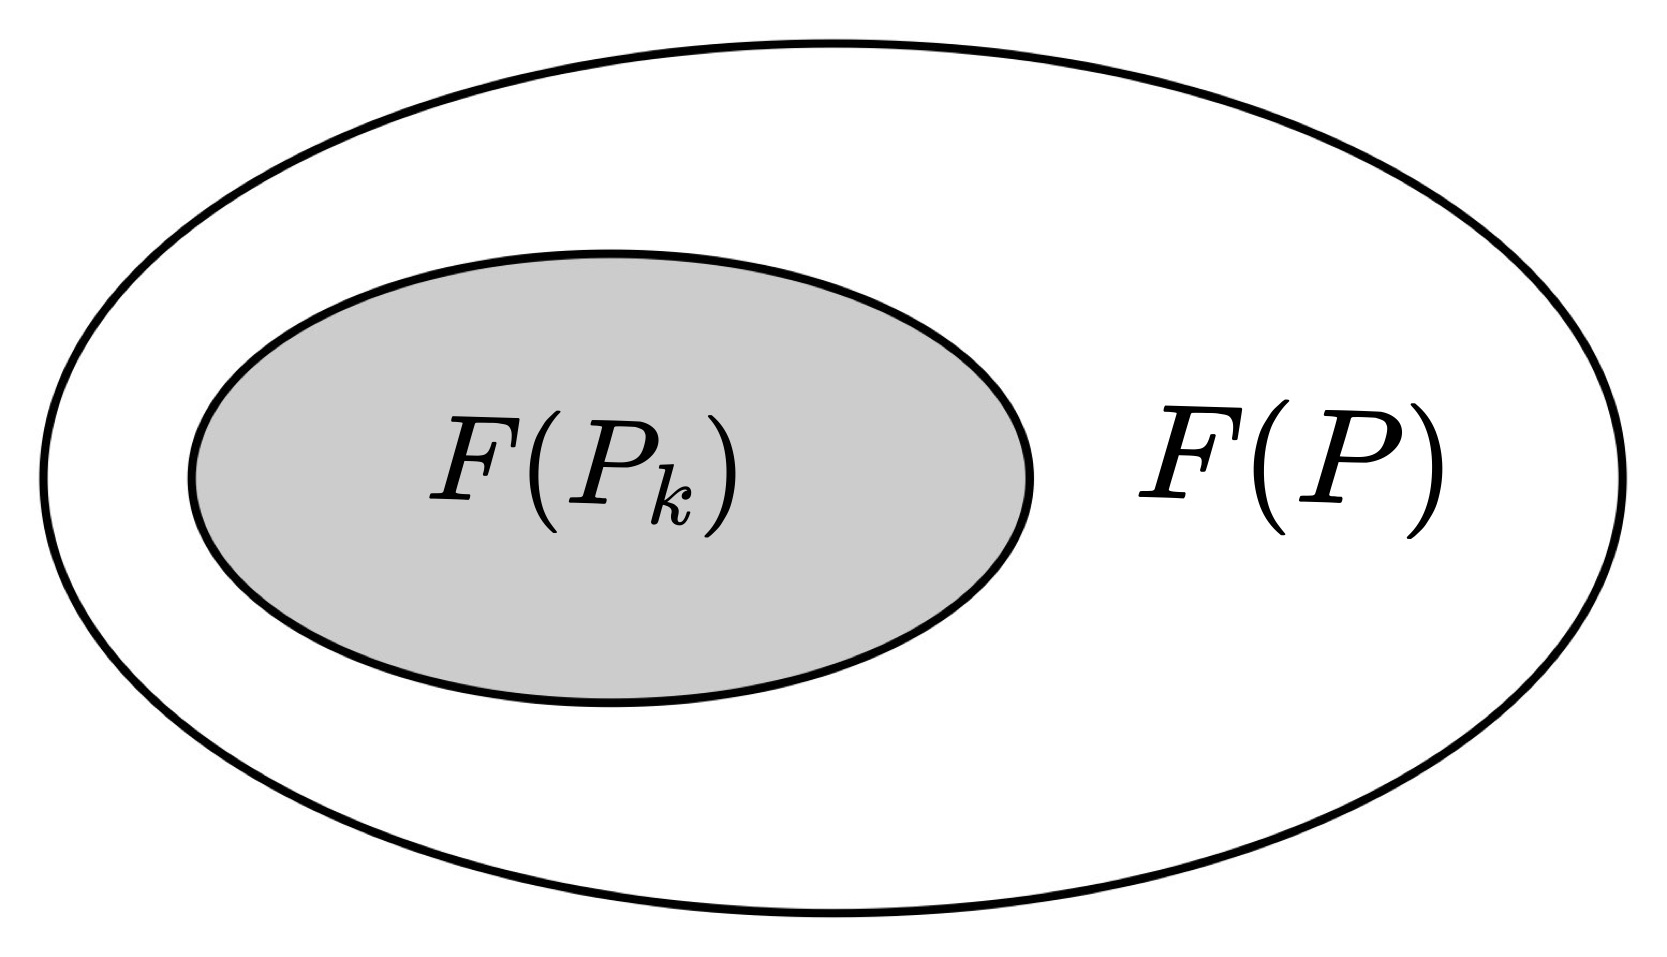
\includegraphics[scale=0.08]{./img/restrizione.jpg}
    \caption{L'insieme delle soluzioni ammissibili di $P_k$ è un
    sottoinsieme dell'insieme delle soluzioni ammissibili di $P$.}
\end{center}
\end{figure}

\noindent
Una ricerca viene detta \textit{esaustiva} quando l'insieme delle restrizioni
$P_k$ ricopre l'intero spazio delle soluzioni ammissibili di $P$, ovvero 
$\bigcup_i F(P_i) = F(P)$.
L'esempio più semplice di algoritmo di ricerca esaustivo è il \textit{generate
and test}.
L'algoritmo ricava tutte le soluzioni $x \in D$, verifica quali di queste
soddisfa i vincoli del problema ed infine sceglie la migliore.
In questo caso le restrizioni di $P$ si ottengono fissando
$x$ ad un certo valore appartenente al dominio $D$.
Per come lo abbiamo descritto, l'algoritmo è esponenziale.
Tuttavia può risultare efficace se utilizzato in casi specifici,
per esempio quando le possibili soluzioni del problema non sono 
in numero elevato e sono computazionalmente poco costose.

Un algoritmo di ricerca esaustiva più avanzato è la \textit{ricerca ad albero}.
L'algoritmo divide ricorsivamente lo spazio di ricerca di $P$ fino ad ottenere
delle restrizioni (corrispondenti alle foglie dell'albero) sufficientemente
facili da risolvere.
Il caso peggiore ha prestazioni esponenziali e si verifica quando tutte le 
foglie corrispondono a restrizioni di $P$ in cui $x$ è fissato ad un valore 
appartenente al dominio $D$, in altre parole l'algoritmo diventa identico
al generate and test.
L'algoritmo per la risoluzione di problemi di programmazione lineare intera 
che introdurremo successivamente, si basa sulla ricerca ad albero.

L'ultima tipologia di ricerca che introduciamo è quella \emph{euristica}.
La ricerca euristica permette di ottenere una soluzione del problema $P$
più velocemente rispetto ad una ricerca esaustiva.
Il vantaggio di questo approccio è proprio la velocità mentre lo svantaggio
principale è che in generale gli algoritmi euristici non sono ottimi, ovvero
non trovano una soluzione ottima ma ne trovano una ammissibile.
L'ACS si basa sulla ricerca euristica.

\subsection{Rilassamento}%
\label{sub:Rilassamento}
Un rilassamento di un problema di ottimizzazione $P$ è un altro problema 
di ottimizzazione $R$ ottenuto da $P$ eliminando alcuni vincoli e sostituendo 
la funzione obiettivo $f(x)$ con una sua approssimazione inferiore $g(x)$.
In altre parole: $R$ è un rilassamento di $P$ se $F(P) \subseteq F(R)$ e se
$g(x) \leq f(x) \quad \forall x \in F(P)$.
Valgono le seguenti proprietà:
\begin{itemize}
    \item se $F(R) = \varnothing$ allora  $F(P) = \varnothing$;
    \item se $x^*$ è una soluzione ottima di $R$, allora $g(x^*)$ è un limite
        inferiore valido per il valore ottimo di $P$.
    \item se $x^*$ è una soluzione ottima di $R$, $x^* \in F(P)$ e $g(x^*) = f(x^*)$,
        allora $x^*$ è ottima anche per $P$.
\end{itemize}

\begin{figure}[ht!]
\begin{center}
    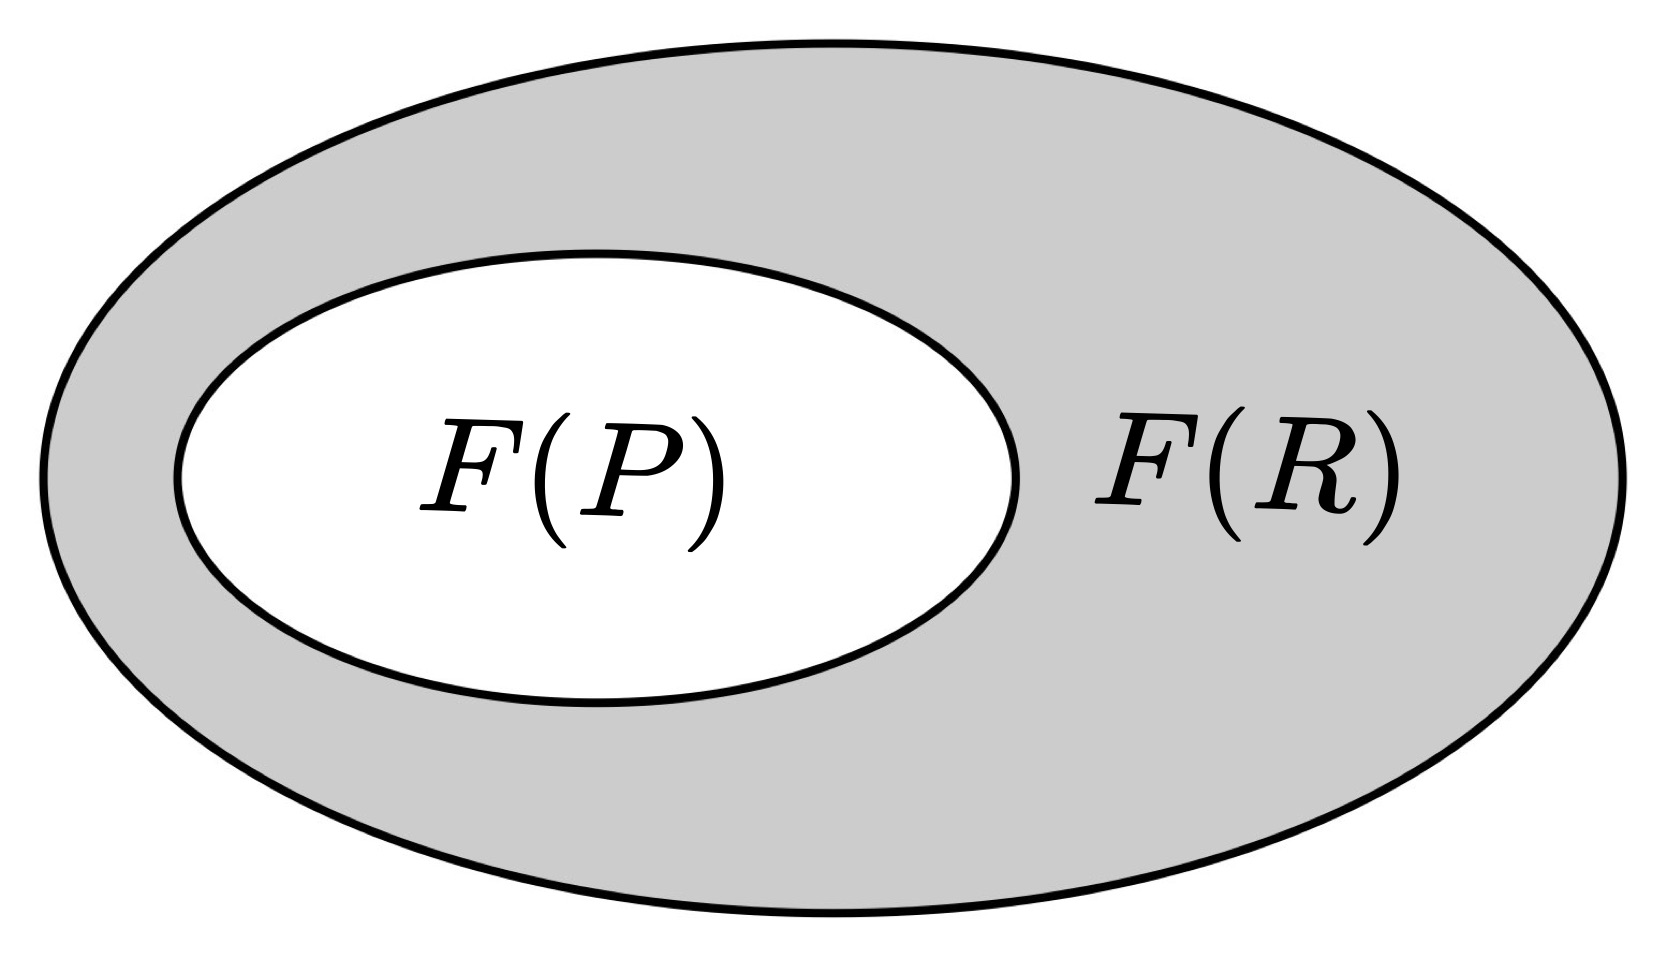
\includegraphics[scale=0.08]{./img/relax.jpg}
    \caption{L'insieme delle soluzioni ammissibili di $P$ è un sottoinsieme
    dell'insieme delle soluzioni ammissibili di $R$.}
\end{center}
\end{figure}

\section{Programmazione lineare}%
\label{sec:Programmazione lineare}
Un generico problema di programmazione lineare è definito come segue:
\begin{equation}
    P:
    \begin{cases}
        \min\,cx\\
        a_ix \sim b_i & i=1,\ldots,m\\
        l_j \leq x_j \leq u_j & j = 1, \ldots, n
    \end{cases}
    \label{eq:lpDef}
\end{equation}
dove $\sim \in \{\leq, \geq, =\}$, $l_j \in \R \cup \{-\infty\}$ e $u_j \in \R \cup 
\{+\infty\}$ e dove $cx$ è funzione lineare.
Le disuguaglianze strette non sono permesse, ciò è dovuto al fatto che 
gli algoritmi che risolvono questa tipologia di problemi richiedono che le 
soluzioni ammissibili appartengano ad un insieme chiuso.
Più avanti vedremo il perché di questa scelta.

Dato un problema di programmazione lineare, esiste un algoritmo che, al caso peggiore,
riesce a risolverlo con complessità polinomiale nella taglia del problema.
La taglia di un problema è definita dal numero delle variabili e di vincoli.

In generale la programmazione lineare è poco applicabile in quanto la maggior
parte dei problemi reali non rientra a far parte di questa categoria.
Sebbene non venga spesso applicata direttamente, risulta essere uno strumento
di fondamentale importanza che viene utilizzato da algoritmi che risolvono
problemi più complessi.

% TODO: Algoritmo del Simplesso.

\section{Programmazione lineare intera}%
\label{sec:MIP intro}
Un problema di programmazione lineare intera (MIP, \emph{Mixed Integer linear 
Programming}) è definito come segue:
\begin{equation}
    P:
    \begin{cases}
        \text{min}\,cx\\
        a_ix \sim b_i & i=1,\ldots,m\\
        l_j \leq x_j \leq u_j & j = 1, \ldots, n = N\\
        x_j \in \Z & \forall j \in J\subseteq N = \{1,\ldots, n\}
    \end{cases}
\end{equation}
dove $\sim \in \{\leq, \geq, =\}$.
Troviamo gli stessi vincoli che si trovano in \ref{eq:lpDef},
in aggiunta è presente il vincolo che alcune delle variabili devono assumere
valori interi.

Si riescono a modellare molti più problemi con la programmazione lineare
intera rispetto alla programmazione lineare.

\subsection{Algoritmo Branch and Bound}%
\label{sub:Algoritmo Branch And Bound}
Il branch-and-bound (B\&B) è un algoritmo che si basa sul paradigma 
divide-and-conquer, viene utilizzato per risolvere problemi di ottimizzazione 
generica tra cui i problemi di programmazione lineare intera.
Il B\&B implementa una ricerca ad albero che permette di 
ricavare una soluzione ottima del problema considerato.

L'algoritmo inizia dal nodo radice il quale rappresenta il problema MIP $P$
che vogliamo risolvere.
\begin{enumerate}
    \item Si considera il rilassamento $R$ di $P$ ottenuto rimuovendo 
        il vincolo di interezza sulle variabili. $R$ è un problema di programmazione 
        lineare ed è quindi più semplice da risolvere.
        Dalle proprietà del rilassamento sappiamo che:
        \begin{enumerate}
            \item Se $F(R) = \varnothing$ allora $F(P) = \varnothing$ quindi
                l'algoritmo termina.
            \item Se esiste una soluzione ottima $x^*\in F(R)$ tale per cui $x^* \in F(P)$,
                allora $x^*$ è ottima per $P$ e l'algoritmo termina.
            \item Se esiste una soluzione $x^*\in F(R)$ tale che $x^* \notin F(P)$,
                ovvero la soluzione trovata non rispetta i vincoli di interezza,
                allora abbiamo trovato un \emph{limite inferiore} sull'ottimo di $P$.
        \end{enumerate}
        Se ci ritroviamo nel caso $(c)$ allora l'algoritmo prosegue.

    \item Si effettua \emph{branching} sul nodo radice.
        L'operazione di branching applicata ad un nodo permette di individuare
        i suoi nodi figli: questi sono sottoproblemi che vengono
        ottenuti mediante restrizioni del problema genitore.
        Almeno una delle variabili della soluzione $x^*$ non rispetta il vincolo
        di interezza, ovvero
        $ \exists\,j \in J \,:\, x^*_j \notin \Z$.
        Di conseguenza due nodi figli possono essere creati imponendo a ciascuno
        uno dei seguenti due vincoli aggiuntivi:
        \begin{equation}
            x_j \leq \lfloor x^*_j \rfloor,\quad x_j \geq \lceil x^*_j \rceil.
        \end{equation}
        I nodi vengono aggiunti alla coda $Q$ dei sottoproblemi da risolvere.
        La Figura~\ref{fig:branching} mostra il risultato di un'operazione di
        branching dal punto di vista della regione ammissibile del problema $P$.
        \begin{figure}[ht!]
            \begin{center}
                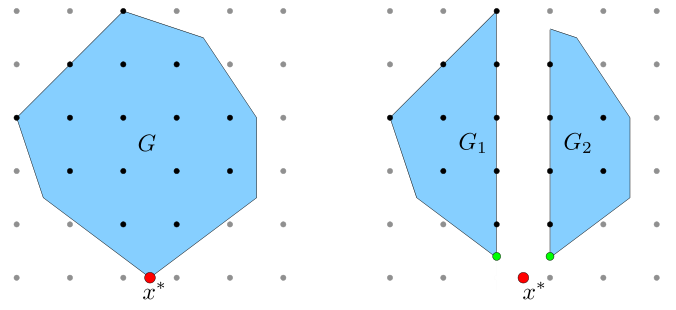
\includegraphics[scale=0.5]{./img/branching.png}
            \end{center}
            \caption{Branching sulla soluzione ottima del rilassamento lineare $x^*$}
            \label{fig:branching}
        \end{figure}

    \item Si procede considerando un sottoproblema $P_i \in Q$ e si risolve
        un suo rilassamento $R_i$.
\end{enumerate}
\begin{itemize}
    \item Quindi i nodi dell'albero sono restrizioni del genitore. 
        Noi risolviamo queste restrizioni tramite rilassamenti.
        Se il rilassamento di un nodo viene impossibile, allora non serve più fare
        branching su quel nodo, possiamo scartarlo (\textbf{pruning by infeasibility}).
        Se il rilassamento mi torna invece un valore intero $\overline{x}$, questo è l'ottimo 
        della restrizione, ed è anche un valore ammissibile per il problema $P$.
        Definiamo $\overline{z}=c\overline{x}$ come l'attuale \textbf{incumbent}: 
        si tratta della miglior soluzione attuale del problema $P$ e per le proprietà
        delle restrizioni è l'upper bound di $P$.
        Questo valore viene aggiornato ogni volta che viene trovato un upper bound 
        migliore (cioè trovo un upper bound più piccolo di quello corrente, considerando
        un problema $P$ di minimizzazione).
    \item Esiste un altro caso in cui possiamo scartare un nodo.
        Se risolvendo il rilassamento di una restrizione trovo una soluzione $x^*$
        che non è intera:
        \begin{itemize}
            \item se $cx^* \geq \overline{z}$ posso scartare
                il nodo; non è necessario fare branching (\textbf{pruning by optimality}).
                Questo perché il rilassamento mi fornisce il lower bound del sottoproblema (nodo),
                di conseguenza anche se risolvessi la restrizione non
                troverei un valore che è più basso di $\overline{z}$ e quindi non ci interessa.
                Questo passo è fondamentale, ci permette di scartare una restrizione senza
                nemmeno risolverla ma risolvendo il rilassamento lineare che per altro
                è molto più semplice e veloce. Questa situazione capita spesso;
            \item se $cx^* < \overline{z}$ allora faccio branching su quel nodo.
        \end{itemize}
    \item Poniamo di bloccare per un istante l'algoritmo e analizziamo la situazione.
        Siamo partiti dalla radice e abbiamo risolto il suo rilassamento; questo 
        ci ha fornito un \textbf{lower bound globale} del nostro problema $P$ e ci ha
        permesso di fare branching; abbiamo ora dei nodi che sono stati scartati e
        altri che devono essere ancora risolti.
        Chiamiamo \textbf{nodi aperti} i nodi che devono essere ancora risolti.
        Sappiamo che risolvendo il rilassamento di un problema otteniamo il lower
        bound di tale problema.
        Adesso: risolvendo i rilassamenti delle restrizioni, otteniamo dei lower
        bound locali che sono riferiti al problema della restrizione, non di 
        quello originale (non sono globali).
        Tuttavia vale una proprietà: se calcoliamo tutti i rilassamenti dei nodi 
        aperti e prendiamo il più piccolo di questi valori, allora questo è un lower bound
        globale.
    \item Da ciò che abbiamo detto al punto precedente apprendiamo che durante
        l'esecuzione dell'algoritmo abbiamo sempre in mano un upper bound $\overline{z}$
        e un lower bound.
        Abbiamo già detto che l'upper bound tende a diminuire.
        Il lower bound viceversa tende ad aumentare.
        Infatti i figli di un nodo sono ottenuti mediante restrizione del padre, quindi
        se il rilassamento del padre mi da un lower bound, i rilassamenti dei due figli 
        non potranno darmi due lower bound più piccoli, sarebbe un assurdo.
        L'algoritmo termina quando non ci sono più nodi aperti, in tale
        situazione si ottiene che l'upper bound coincide con il lower bound,
        cioè abbiamo trovato l'ottimo di $P$ e abbiamo dimostrato che non si può
        fare meglio di così (figura~\ref{fig:andamentoUpperLowerBound}).
\end{itemize}

\begin{figure}[ht!]
\begin{center}
    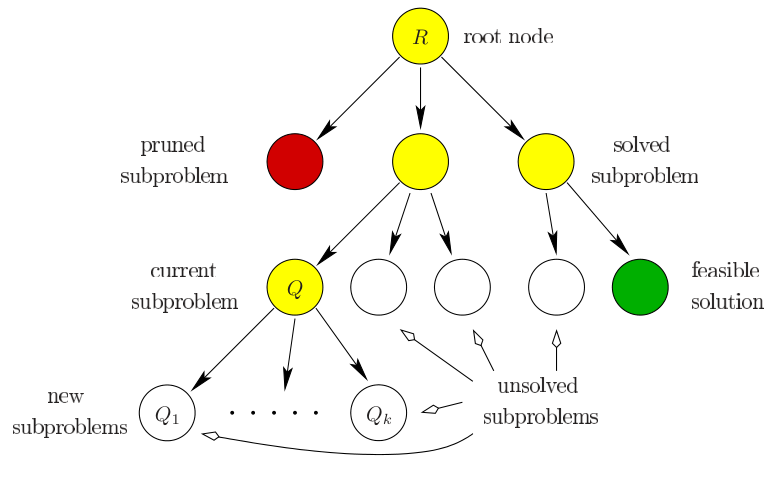
\includegraphics[scale=0.4]{./img/branchandbound.png}
\end{center}
\caption{Ricerca ad albero di un algoritmo B\&B}
\end{figure}

\begin{figure}[ht!]
\begin{center}
    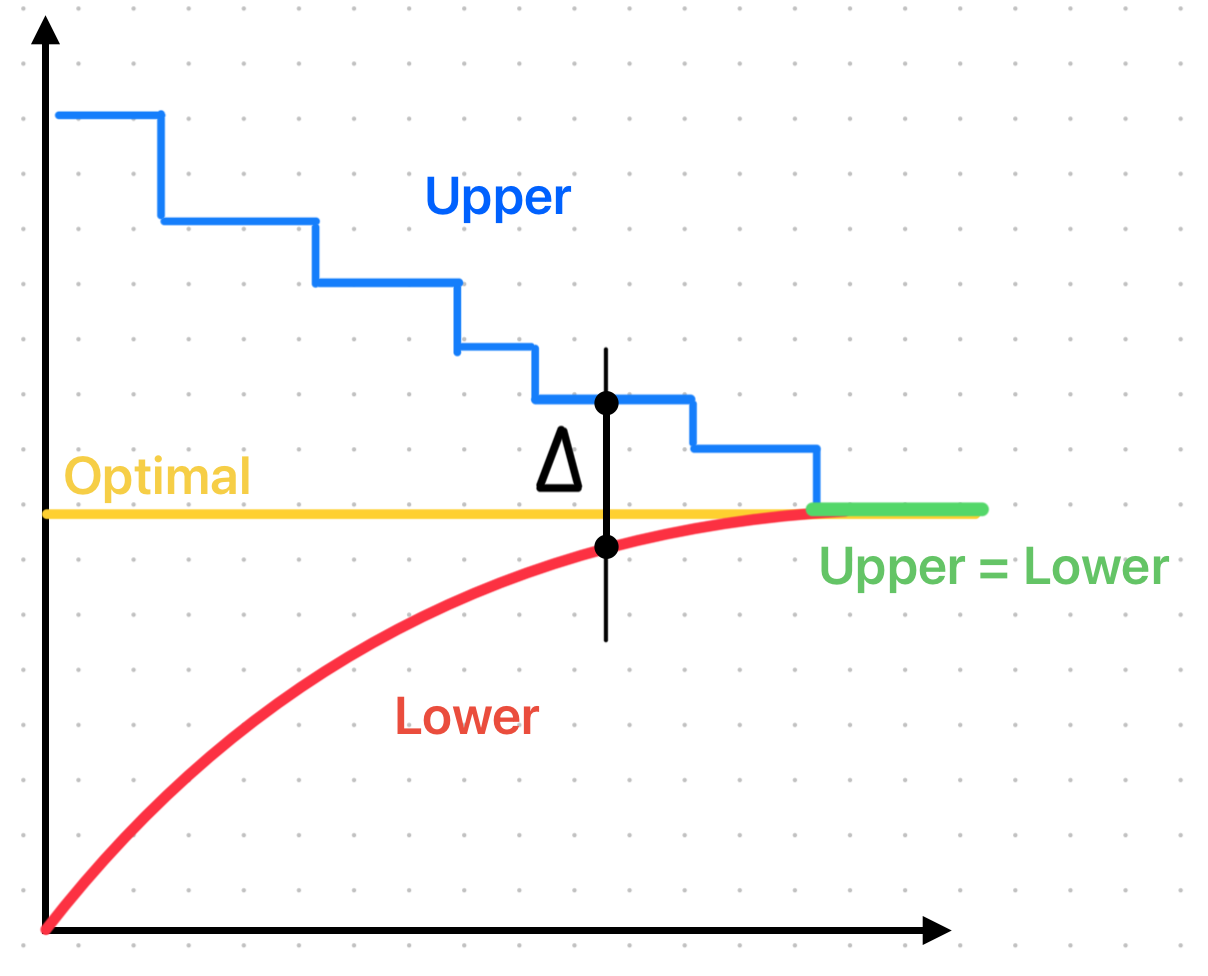
\includegraphics[scale=0.45]{./img/bnbLowerUpperBound.png}
\end{center}
\caption{Andamento dell'upper e del lower bound nel tempo nell'algoritmo B\&B}
\label{fig:andamentoUpperLowerBound}
\end{figure}

Visto che l'algoritmo memorizza l'upper bound e il lower bound ad ogni istante,
allora potremmo decidere di non far terminare l'algoritmo quando questi due valori
coincidono, possiamo specificare un $\Delta = $ upper - lower  entro il quale
fermarsi.
Questo ci permette di trovare un range entro il quale si trova certamente la soluzione
ottima del problema.
In base all'applicazione e al problema che stiamo considerando potremmo voler 
restringere il valore del $\Delta$. 
Ovviamente il vantaggio di avere un delta che non è $\Delta = 0$ (che per $t \to +\infty$ 
verrebbe raggiunto) sono i tempi computazionali.

\section{Algoritmo Branch and Cut}%
\label{sec:Algoritmo Branch and Cut}
L'algoritmo B\&C è una versione migliorata dell'algoritmo B\&B sviluppata 
specificatamente per il caso MIP.
L’algoritmo B\&C è essenzialmente un algoritmo ibrido B\&B/piani di taglio, basato 
sulla seguente semplice idea: ad ogni nodo dell'albero decisionale, la formulazione 
associata al rilassamento del sottoproblema corrente può essere rafforzata mediante 
la generazione di piani di taglio.
Il rafforzamento viene fatto per due motivi:
\begin{itemize}
    \item per ottenere una soluzione intera del rilassamento lineare;
    \item per ottenere un lower bound migliore quindi più efficace per il pruning.
\end{itemize}
Si tratta di una tecnica molto efficace che migliora notevolmente le prestazioni rispetto
all'algoritmo B\&B e ai piani di taglio puri.

\begin{figure}[ht!]
\begin{center}
    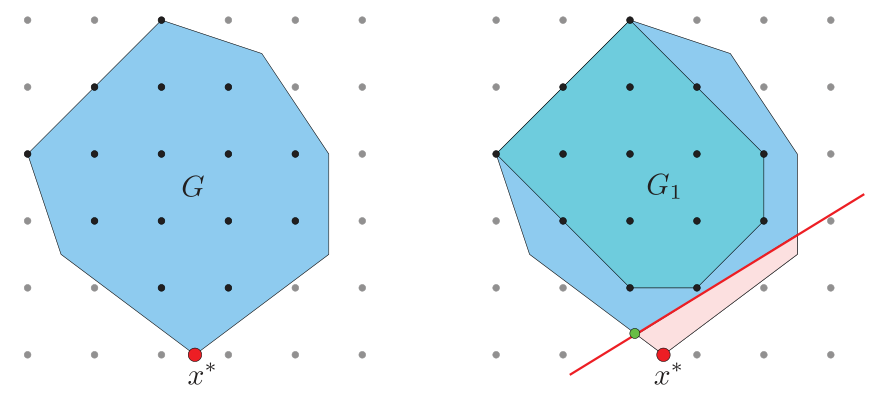
\includegraphics[scale=0.4]{./img/branchandcut.png}
\end{center}
\caption{Rafforzamento di un rilassamento mediante piani di taglio}
\end{figure}

\section{Modellazione MIP}%
\label{sec:Modellazione MIP}
Vediamo quali tipi di problemi possiamo modellare sfruttando il paradigma della
programmazione lineare intera.

\subsection{Decisioni y/n}%
\label{sub:Decisioni y/n}
Con la programmazione ciò era impossibile. In
MIP possiamo sfruttare le variabili binarie (assumono valori $\in \{0,1\}$)
per questo scopo.

\subsection{Variabili discrete}%
\label{sub:Variabili discrete}
Si intendono non solo variabili intere ma variabili
che hanno un numero finito di valori ammissibili (anche non numerici):
Andremmo ad introdurre quindi
\[ 
    y \in \{s_1,\ldots,s_m\}
\]
e l'obbiettivo sarà scegliere una tra le $m$ possibilità.
Anche in questo caso sfrutteremo delle variabili binarie descritte come segue
\[
    x_i =
    \begin{cases}
        1 & \text{se } y= s_i\\ 
        0 & \text{altrimenti}
    \end{cases}
\]
Il problema sarà allora definito come segue
\[
    \begin{cases}
        y = \sum^{m}_{i = 1} s_i x_i\\
        \sum^{m}_{i=1} x_i = 1 \quad \text{(per avere un'unica scelta)}\\
        x_i \in \{0,1\}
    \end{cases}
\]

\subsection{Costi fissi}%
\label{sub:Costi fissi}
Immaginiamo di avere
\[
    0\leq x \leq u,\quad c(x) =
    \begin{cases}
        ax + b & \text{se } x > 0\\
        0 & \text{se } x = 0\\
    \end{cases}
\]
cioè abbiamo definito la funzione dei costi che dipende dalla quantità di
prodotto $x$.
Notiamo che $c(x)$ è una funzione lineare continua a tratti.
Per trattare questo tipo di problemi conviene introdurre una variabile
binaria per separare i due casi:
\[
    y =
    \begin{cases}
        1 & \text{se } x > 0 \\ 
        0 & \text{se } x = 0
    \end{cases}
\]
Il modello del problema diventa il seguente
\[
    \begin{cases}
        c(x,y) = ax + by\\
        0 \leq x \leq uy\\
        y \in \{0,1\}
    \end{cases}
\]
per verificare la correttezza conviene sempre andare a sostituire $y$ con
$0$ poi con $1$ e controllare che tutto torni.
Quindi:
\[
    y = 0 \Rightarrow
    \begin{cases}
        c(x) = ax\\
        x = 0
    \end{cases}
    \Rightarrow c(x) = 0
\]
Corretto.
\[
    y = 1 \Rightarrow
    \begin{cases}
        c(x) = ax + b\\
        0 \leq x \leq u
    \end{cases}
\]
Questo caso non è esattamente quello che vogliamo: anche in questo caso potremmo
avere che $x = 0$  quando $y = 1$. 
Situazione che abbiamo escluso in precedenza.
Come facciamo in questi casi?
Esistono diverse soluzioni che dipendono dal problema:
\begin{itemize}
    \item In molti contesti si dimostra che, anche se $y = 1$, $x = 0$ è 
        ammissibile, non è mai soluzione ottima.
        Ciò va dimostrato caso per caso.
    \item In altri casi viene dato un lower bound oltre che un upper bound.
        In tal caso la funzione $c(x)$ viene definita come segue
        \[
            c(x) =
            \begin{cases}
                ax + b & \text{se } x > \varepsilon\\
                0      & \text{se } x = 0
            \end{cases}
        \]
        e quindi il problema non sussiste.
    \item Se su $x$ vige il vincolo di interezza, allora si può
        porre banalmente come lower bound $\varepsilon = 1$ e si
        risolve il problema.
\end{itemize}

\begin{figure}[ht!]
\begin{center}
    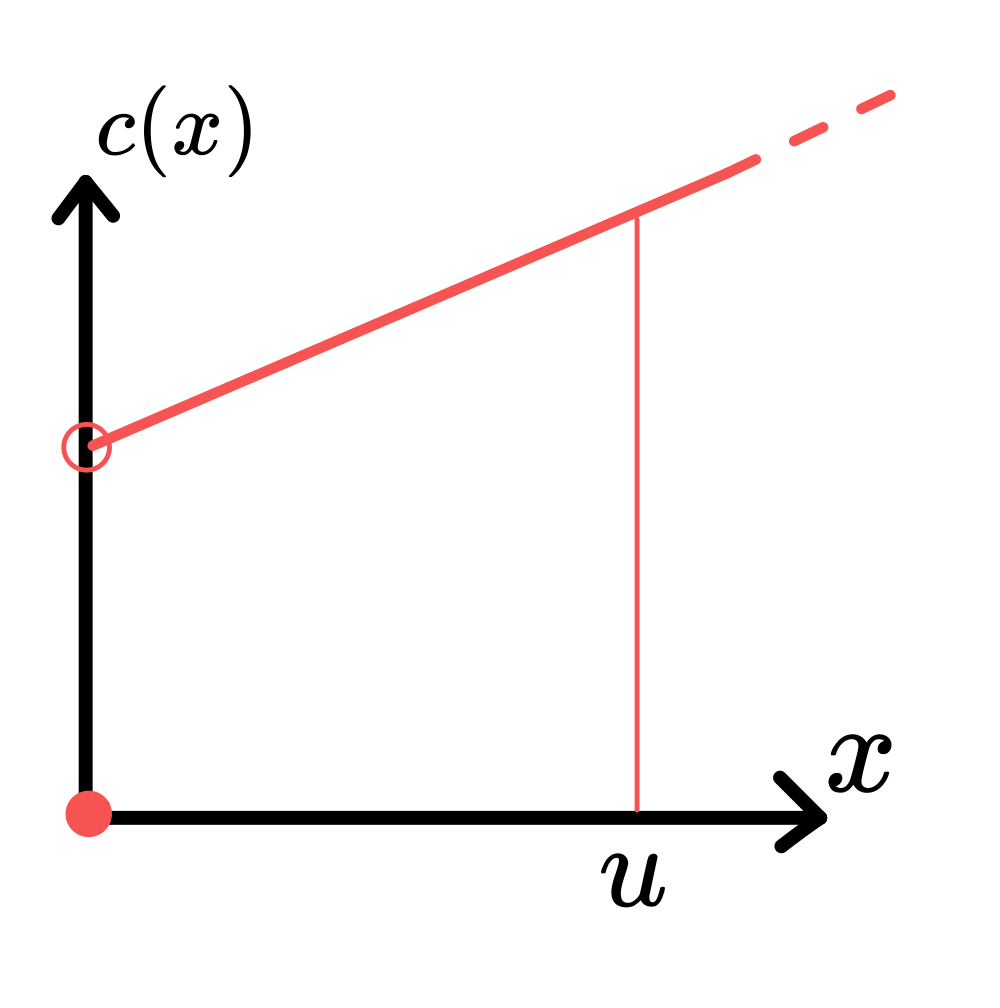
\includegraphics[scale=0.2]{./img/costiFissi.png}
\end{center}
\caption{Grafico della funzione $c(x)$}
\label{fig:esCostiFissi}
\end{figure}

\subsection{Disgiunzioni}%
\label{sub:Disgiunzioni}
Fino ad ora i vincoli di un problema dovevano essere
soddisfatti tutti.
Nelle disgiunzioni si richiede che almeno uno venga soddisfatto.
Per esempio se i vincoli sono due, possiamo dire che almeno uno di
essi venga soddisfatto come segue (usiamo una OR):
\[
    (a_1 x \leq b_1) \vee (a_2 x \leq b_2)
\]
Vediamo come modellare questo tipo di problemi usando al solito delle
variabili binarie (una per ogni vincolo).
Poniamo:
\[
    l\leq x \leq u, \quad y_i =
    \begin{cases}
        1 & \text{se } a_i x \leq b_i\\
        0 & \text{altrimenti}
    \end{cases}
\]
Il problema diventa:
\[
    \begin{cases}
        a_1 x \leq b_1 + M(1-y_1)\\ 
        a_2 x \leq b_2 + M(1-y_2)\\ 
        y_1 + y_2 \geq 1 \\
        y_i \in \{0,1\} \\
        l \leq x \leq u
    \end{cases}
\]
in questo modo, attraverso $y_i$ e $M$ (detta \emph{big M}) possiamo attivare
un vincolo e disattivare l'altro e non possono mai essere entrambi disattivi
visto che la somma degli $y_i$ deve essere $\geq1$.
Il termine $M$ serve per indicare che esiste un certo valore sufficientemente 
grande che soddisfa il vincolo, cioè permette di renderlo ridondante.
Il fatto che $x$ sia bounded ci permette di affermare che esiste un tale
valore di $M$.
Si tratta ora di capire che valore assegnare ad $M$: se è troppo grande di fatto
andiamo a disattivare entrambi i vincoli e il rilassamento sul problema diventa debole;
ci serve che $M$ sia il più piccolo
necessario.

Vediamo un semplice esempio di problema che possiamo modellare con le disgiunzioni.
Vediamo l'esempio del valore assoluto:
\[
    \begin{cases}
        \abs{x-2} \geq 1 \leadsto x - 2 \geq 1 \vee x - 2 \leq -1 \\
        0 \leq x \leq 4
    \end{cases}
\]
sfruttando le disgiunzioni il modello è il seguente:
\[
    \begin{cases}
        x \geq 3y \\
        x \leq 1 + 3y \\
        y \in \{0,1\}\\
        0 \leq x \leq 4 
    \end{cases}
\]

\begin{figure}[ht!]
\begin{center}
    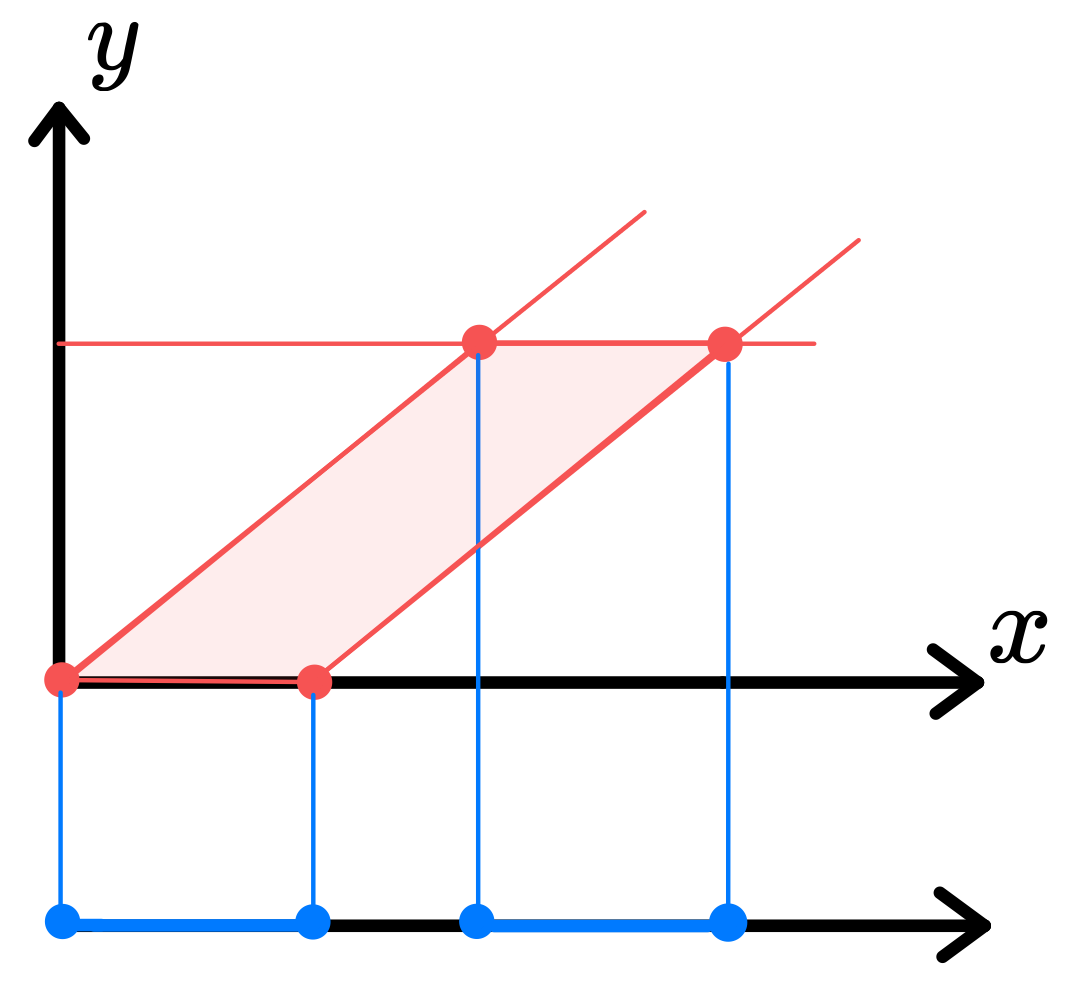
\includegraphics[scale=0.17]{./img/disgiunzioneValAssoluto.png}
\end{center}
\caption{Proiezione del dominio delle soluzioni sul dominio della variabile $x$}
\label{fig:esempioValAssoluto}
\end{figure}

Dalla figura~\ref{fig:esempioValAssoluto} vediamo come, con le disgiunzioni, sia
possibile modellare problemi che non sono convessi nello spazio originario.

\subsection{Funzioni lineari a tratti}%
\label{sub:Funzioni lineari a tratti}
Vogliamo descrivere un modello MIP di una funzione lineare a tratti.
Questo tipo di funzioni potrebbe essere presente nei problemi in cui per esempio
si cerca di approssimare una funzione non lineare.
Partiamo dal fatto che una funzione lineare a tratti è univocamente determinata
dai punti della spezzata.
Identifichiamo questi con i punti $a_1,\ldots,a_k$ e $f(a_1),\ldots,f(a_k)$.
Notiamo che gli intervalli presi singolarmente sono lineari; il problema è che non
sappiamo in che intervallo siamo ma sappiamo che $x$ deve assumere uno dei valori
presenti nei vari intervalli.
Quindi $x$ deve cadere in uno degli intervalli, che sono in numero finito, sono $k-1$.
Ciò significa che possiamo introdurre delle variabili binarie $y_i$ che scelgano l'intervallo,
similmente a come abbiamo fatto in precedenza nei problemi con variabili discrete.

\begin{figure}[ht!]
\begin{center}
    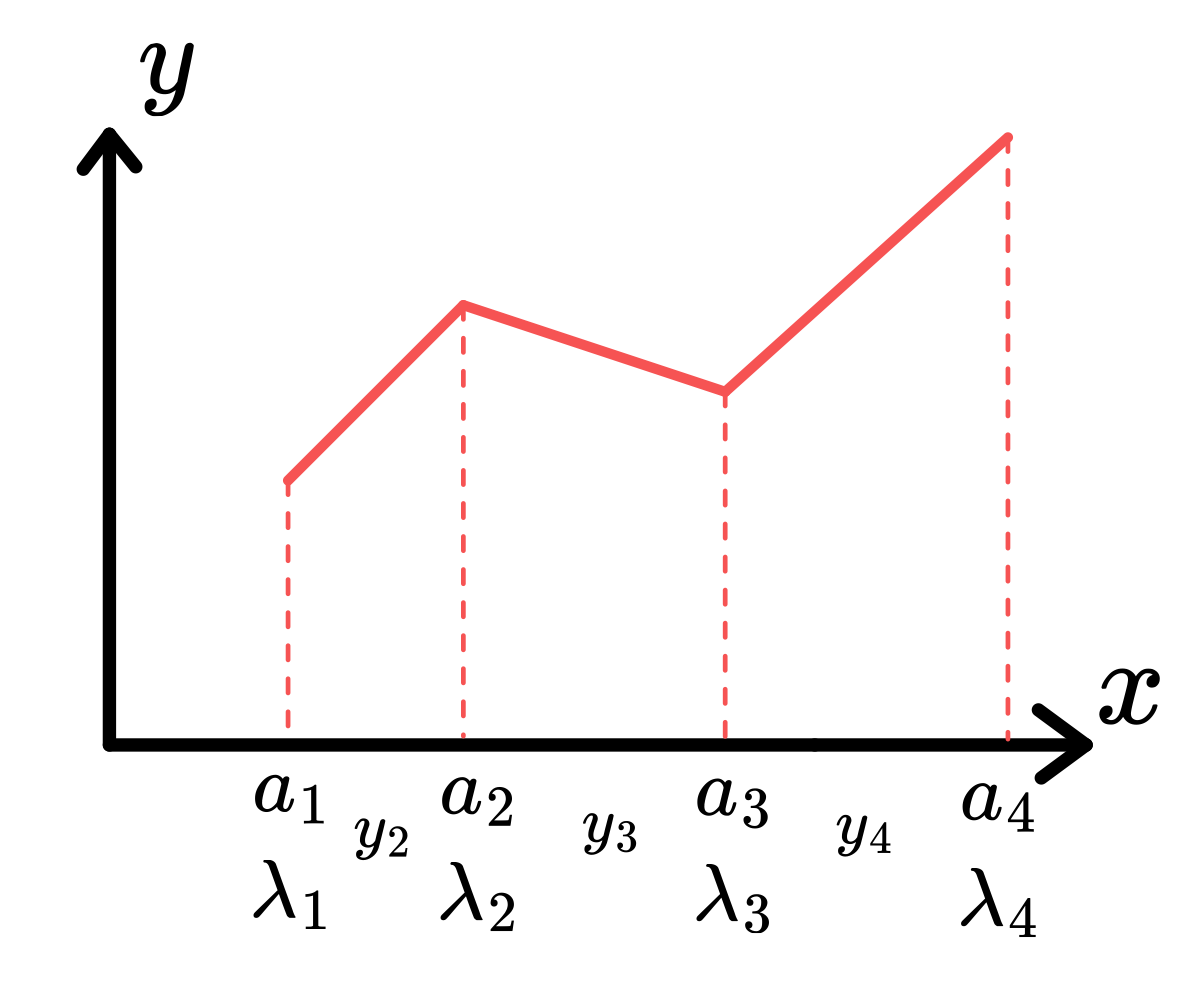
\includegraphics[scale=0.2]{./img/funzLinTratti.png}
\end{center}
\caption{Funzione lineare a tratti}
\end{figure}

\[
    \begin{cases}
        \sum^{k}_{i=1} y_i = 1 \\
        x = \sum^{k}_{i=1} \lambda_i a_i \\
        c(x) = \sum^{k}_{i=1} \lambda_i c(a_i) \\
        y\in \{0,1\} & i = 1,\ldots k-1 \\
        \lambda_i \geq 0 & i = 1,\ldots k \\
        \sum^{k}_{i=1} \lambda_i = 1 \\
        \lambda_1 \leq y_1 \\
        \lambda_i \leq y_{i-1} + y_i & i = 2,\ldots,k-1 \\
        \lambda_k \leq y_{k-1}
    \end{cases}
\]
dove in particolare:
\begin{itemize}
    \item $\sum^{k}_{i=1} y_i = 1$ mi impone che devo stare in un unico intervallo;
    \item i $\lambda_i$ sono i moltiplicatori (variabili continue$\in [0,1]$) che mi permettono 
        di esprimere tutti i punti che si trovano tra i due estremi di un segmento.
        Infatti i punti di un segmento possono essere espressi come combinazione
        convessa dei suoi estremi.
        Abbiamo detto che dobbiamo scegliere un segmento per volta e ciò comporta
        che dobbiamo anche vincolare l'uso dei moltiplicatori $\lambda_i$ corretti,
        gli altri devono essere uguali a zero.
        Otteniamo questo comportamento imponendo i vincoli $\lambda_1 \leq y_1$, 
        $\lambda_i \leq y_{i-1} + y_i$, $\lambda_k \leq y_{k-1}$.
\end{itemize}

\subsection{Set covering e set partitioning}%
\label{sub:Set covering e set partitioning}
Nei problemi di \textbf{set covering} individuiamo
\[
    I \text{ grand set}, \quad F = \{F_1,\ldots, F_N\} \text{ famiglia}\quad 
    F_i \subseteq I \quad  i = 1,\ldots, N 
\]
si tratta di trovare il minimo $N$ tale che l'unione degli insiemi $F_i$ ricopra
interamente l'insieme $I$.
Si tratta dunque di introdurre delle variabili binarie
\[
    x_j =
    \begin{cases}
        1 &\text{se scelgo } F_j\\
        0 &\text{altrimenti}
    \end{cases}
\]
il modello dunque diventa il seguente
\[
    \begin{cases}
        \text{min}\, \sum_{j=1}^N x_j \\
        \sum_{j=1}^N x_j \geq 1 & \forall i \in I\\
        x_j \in \{0,1\} & \forall j \in J
    \end{cases}
\]
I problemi di \textbf{set partitioning} si modellano in maniera simile:
\[
    \begin{cases}
        \text{min}\, \sum_{j=1}^N x_j \\
        \sum_{j=1}^N x_j = 1 & \forall i \in I\\
        x_j \in \{0,1\} & \forall j \in J
    \end{cases}
\]

Notiamo che nel caso di problemi di set covering, è semplice trovare una soluzione
ammissibile (basta settare tutte le variabili binarie a $1$), ma risulta difficile
trovare la soluzione ottima.
I problemi di set partitioning sono in generale più complicati e per questo spesso
si decide di risolvere il rilassamento al set covering.

\subsection{Max stable set}%
\label{sub:Max stable set}
\begin{definition}[Stable set]
   Dato un grafo $G = (V,E)$, un sottoinsieme di nodi $S\subseteq V$ si dice 
   stabile se
   \[
       \forall i,j \in S\quad (i,j) \notin E
   \]
\end{definition}

\noindent
Facendo riferimento alla figura~\ref{fig:esempioDiGrafo}, il max stable set 
del grafo riportato è $S=\{1,4,5,6\}$.

Si tratta di trovare l'insieme stabile con cardinalità maggiore di un grafo dato.
Dunque dobbiamo decidere, per ogni nodo, se questo entra a far parte del set
oppure no.
Utilizziamo a tale scopo delle variabili binarie.
\[
    x_i =
    \begin{cases}
        1 &\text{se nodo } i\in S \\
        0 &\text{altrimenti}
    \end{cases}
\]
Il modello diventa
\[
    \begin{cases}
        \text{max}\, \sum_{i\in V} x_i\\
        x_i + x_j \leq 1 & \forall (i,j) \in E\\
        x_i \in \{ 0,1\} & \forall i \in V
    \end{cases}
\]
dove il primo vincolo impone che al massimo uno dei due nodi estremi di un arco
possa essere inserito nell'insieme $S$.


\subsection{Max clique set}%
\label{sub:Max clique set}
Si tratta del problema complementare al quello dell'individuare il max stable set.
\begin{definition}[Clique set]
   Dato un grafo $G = (V,E)$, un sottoinsieme di nodi $S\subseteq V$ si dice 
   clique se
   \[
       \forall i,j \in S\quad (i,j) \in E
   \]
\end{definition}

\noindent
Facendo riferimento alla figura~\ref{fig:esempioDiGrafo}, il max clique set 
del grafo riportato è $S=\{2,3,4\}$.

Vale la seguente \textbf{proprietà}:
\[
    S \text{ è un clique set di } G=(V,E)\Leftrightarrow S \text{ è uno stable set di }
    \overline{G} = (V,\overline{E}).
\]
Sfruttando tale proprietà, il problema si traduce nell'individuare il max stable
set del grafo complementare a quello dato.
Il modello dunque è il seguente
\[
    \begin{cases}
        \text{max}\, \sum_{i\in V} x_i\\
        x_i + x_j \leq 1 & \forall (i,j) \in \overline{E}\\
        x_i \in \{ 0,1\} & \forall i \in V
    \end{cases}
\]
Matematicamente il concetto è corretto, possiamo sfruttare la proprietà enunciata
e risolvere il modello che abbiamo scritto.
Il problema è che se il grafo ha densità bassa\footnote{La densità di un grafo
è data dal rapporto tra numero di archi e numero di coppie di nodi.}, 
il suo complementare ha un elevata densità e ciò può provocare problemi di memoria
se il grafo di partenza ha una dimensione elevata.

\begin{figure}[ht!]
\begin{center}
    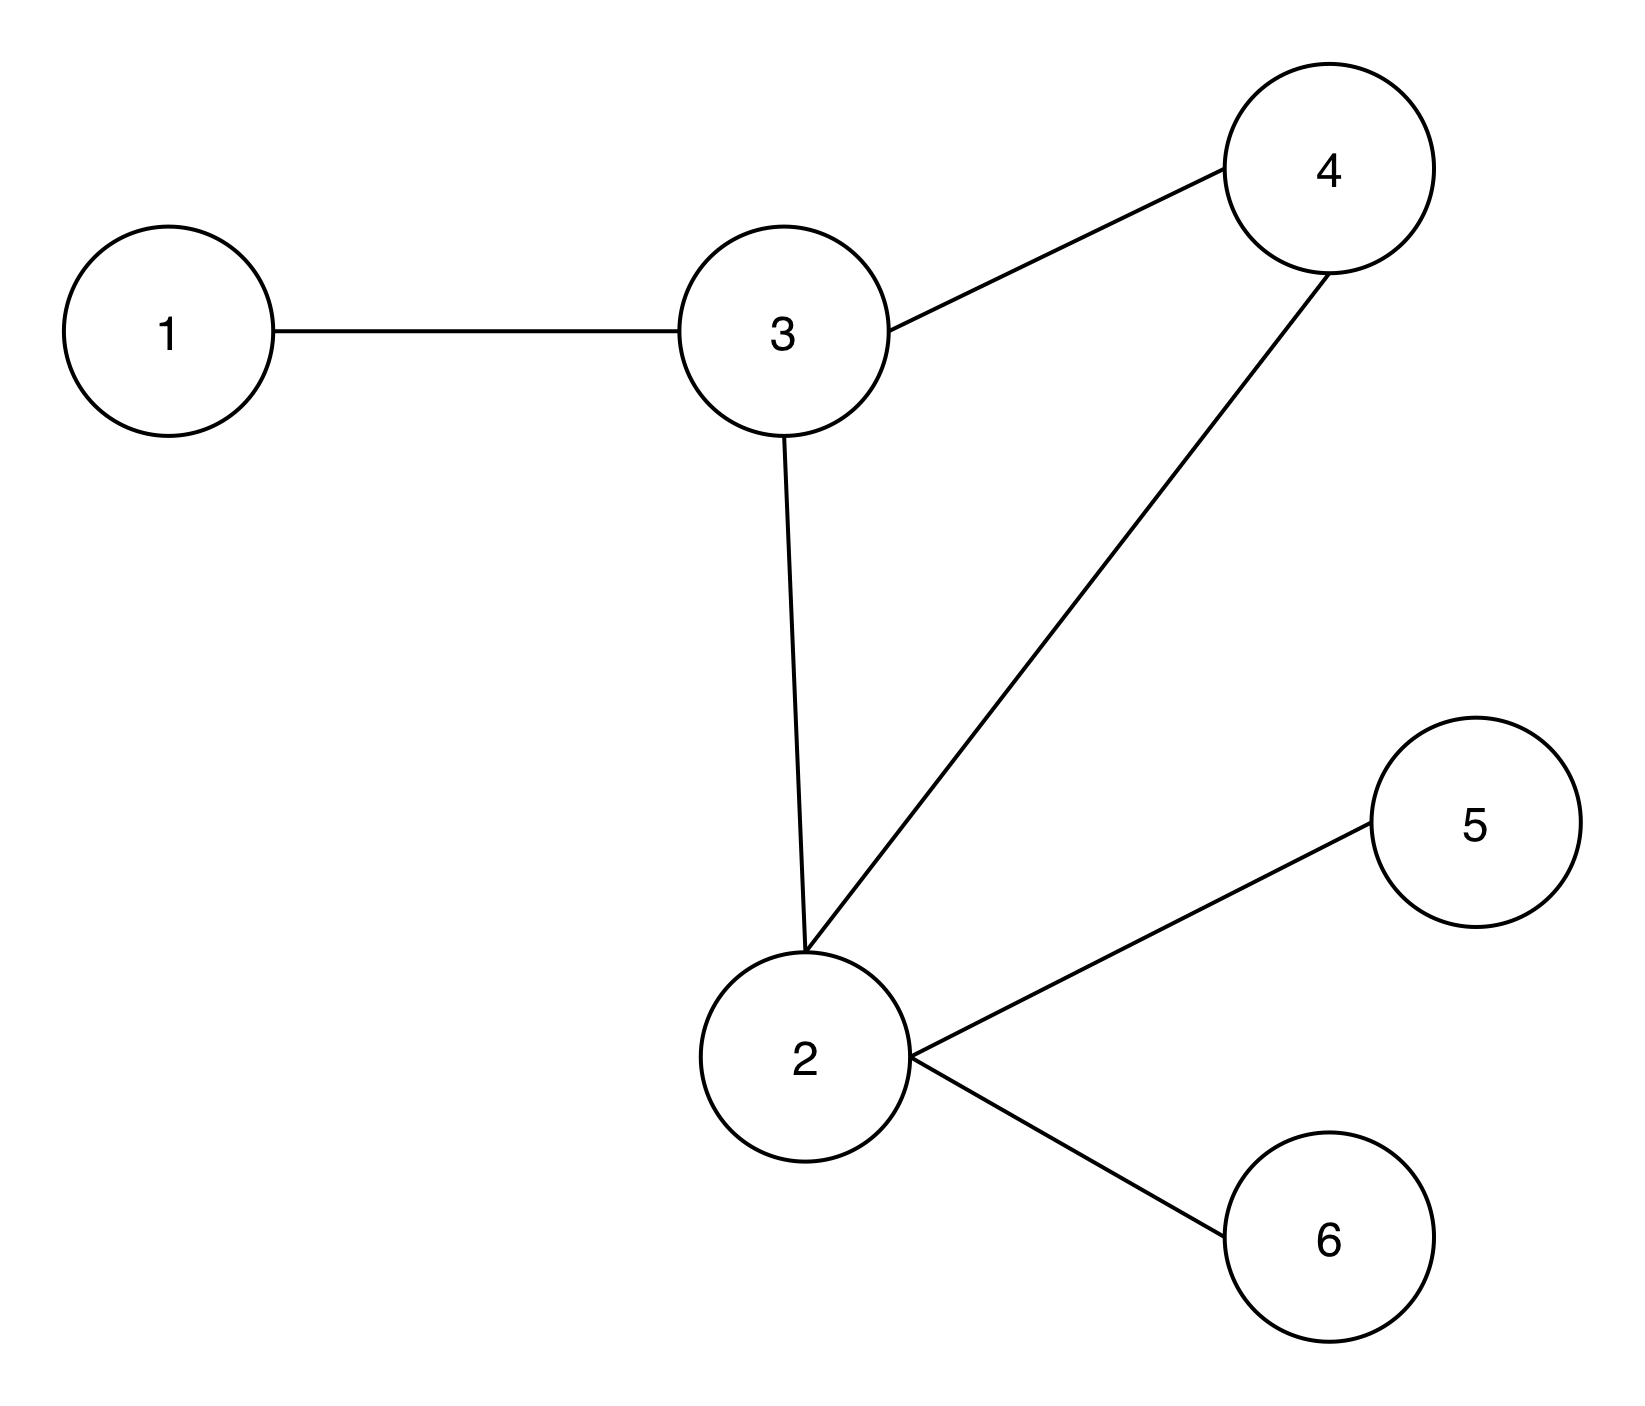
\includegraphics[scale=0.55]{./img/graph.png}
\end{center}
\caption{Un grafo}
\label{fig:esempioDiGrafo}
\end{figure}

\subsection{Vertex coloring}%
\label{sub:Vertex coloring}
Si tratta di problemi in cui ci viene dato un grafo e il nostro obbiettivo è 
quello di riuscire a colorare i vertici in modo tale che due vertici adiacenti
non abbiamo lo stesso colore.
I problemi di vertex coloring hanno due verioni, vediamole entrambe.

Nella \textbf{versione di ammissibilità}: ci viene dato un insieme di colori
e dobbiamo dire se con questi riusciamo a colorarlo senza che vertici adiacenti
abbiamo lo stesso colore.
La risposta dell'algoritmo risolutivo sarà affermativa o negativa.
Come modelliamo il problema per questa versione?
\[
    \text{Colori = }\{1,\ldots,K\},\quad x_i := \text{ colore da assegnare
    al nodo } i
\]

\[
    \begin{cases}
        x_i \neq x_j & \forall (i,j) \in E\\
        x_i \in \{1,\ldots,K\} & \forall i \in V
    \end{cases}
\]
Sebbene sia matematicamente corretto, non è MIP a causa del $\neq$.
Ovviamo all'utilizzo del $\neq$ modellando in maniera differente.
Introduciamo delle variabili binarie:
\[
    x_{i,k} = 
    \begin{cases}
        1 & \text{se nodo $i$ ha colore $k$}\\
        0 & \text{altrimenti}
    \end{cases}
\]
il modello è il seguente
\[
    \begin{cases}
        x_{i,k} + x_{j,k} \leq 1 & \forall (i,j) \in E \quad \forall k = 1,\ldots,K\\
        \sum^{K}_{k=1} x_{i,k} = 1 & \forall i \in V\\
        x_{i,k} \in \{0,1\} & \forall i \in V\quad \forall k = 1,\ldots,K
    \end{cases}
\]
dove: il primo vincolo impone che nodi adiacenti abbiano colori diversi; 
il secondo vincolo impone che tutti i nodi del grafo siano colorati.

Nella \textbf{versione di ottimizzazione}: non ci viene dato l'insieme dei colori;
il problema consiste nel trovare il minor numero di colori da utilizzare affinché
il grafo non presenti nodi adiacenti con lo stesso colore.
L'upper bound del problema è dunque uguale al numero di nodi del grafico, che poniamo
sia $N$.
Si utilizzano $N$ colori quando si ha che ogni nodo del grafo è connesso a tutti
gli altri nodi.
Introduciamo
\[
    \begin{split}
        w_k & =
        \begin{cases}
            1 & \text{se uso il colore $k$}\\
            0 & \text{altrimenti}
        \end{cases}
        \quad \forall k \in K = \{1, \ldots, N\}
        \\
        x_{i,k} & = 
        \begin{cases}
            1 & \text{se nodo $i$ ha colore $k$}\\
            0 & \text{altrimenti}
        \end{cases}
    \end{split}
\]
il modello è il seguente
\[
    \begin{cases}
        \text{min}\,\sum^{N}_{k=1} w_k\\
        \sum^{N}_{k=1} x_{i,k} = 1 & \forall i \in V\\
        x_{i,k} + x_{j,k} \leq w_k & \forall(i,j)\in E \quad \forall k = 1,\ldots, N\\
        x_{i,k} \in \{0,1\} & \forall i \in V\\
        w_k\in \{0,1\} & k = 1,\ldots,N
    \end{cases}
\]
dove il secondo vincolo 
mette in relazione le variabili binarie $x_{i,k}, w_k$ e impone
che i nodi adiacenti abbiano colori diversi.

\subsection{Facility location}%
\label{sub:Facility location}
In questo tipo di problemi abbiamo due insiemi: una lista di facilities che
devo decidere se creare/aprire; una lista di clienti da associare alle facilities
create/aperte.

Per esempio poniamo di dover interrogare un data base relazionale: abbiamo $n$ query 
(clients) da fare e $m$ indici che possiamo creare.
Per ogni indice, una query ha un costo (in termini di tempi di risposta) pari
a $c_{ij}$ e inoltre creare un indice ha un costo fisso di $c_j$.
Si tratta di scegliere quale indice creare e quale (tra quelli creati)
usare per ogni query.
Introduciamo allora delle variabili binarie:
\[
    \begin{split}
        x_{ij} & =
        \begin{cases}
            1 & \text{se la query $i$ usa l'indice $j$}\\
            0 & \text{altrimenti}
        \end{cases}
        \\
        y_j & =
        \begin{cases}
            1 & \text{se creo l'indice }j \\
            0 & \text{altrimenti}
        \end{cases}
        \end{split}
\]
il modello è il seguente
\[
    \begin{cases}
        \text{min}\, \sum_{i\in I} \sum_{j\in J} c_{ij} x_{ij} + \sum_{j\in J} c_j y_j \\
        \sum_{j\in J} x_{ij} = 1 & \forall i \in I\\
        x_{ij} \leq y_{j} & \forall i \in I,\, \forall j \in J \\
        x_{ij} \in \left\{ 0,1 \right\}, \quad y_j \in \left\{ 0,1 \right\}
    \end{cases}
\]
dove: il primo vincolo impone che venga scelto esattamente un indice per ogni query;
il secondo vincolo impone che la scelta dell'indice da usare per ogni query
sia uno tra quelli disponibili, cioè tra quelli creati.

\subsection{Knapsack}%
\label{sub:Knapsack}
Nel classico problema del knapsack abbiamo uno zaino con una capienza $C$ fissata
e un insieme di oggetti che hanno un peso $w_i$ e un profitto associato $p_i$.
L'obiettivo è quello di riempire lo zaino in modo tale massimizzare il profitto.
Si tratta quindi di scegliere quale oggetto mettere nello zaino.
\[
    x_i =
    \begin{cases}
        1 &\text{se l'oggetto $i$ lo metto nello zaino}\\
        0 &\text{altrimenti}
    \end{cases}
\]
il modello è il seguente
\[
    \begin{cases}
        \text{max } \sum_{i \in I} p_i x_i\\
        \sum_{i \in I} w_i x_i \leq C\\
        x_i \in \{0,1\} & \forall i \in I
    \end{cases}
\]
Una variante dello stesso problema è il knapsack multiplo: la differenza è che
abbiamo un insieme $J$ di zaini, ognuno con la sua capacità $C_j$.
\[
    x_{ij} =
    \begin{cases}
        1 &\text{se l'oggetto $i$ lo metto nello zaino $j$}\\
        0 &\text{altrimenti}
    \end{cases}
\]
\[
    \begin{cases}
        \text{max } \sum_{i\in I} \sum_{j\in J} p_i x_{ij}\\
        \sum_{i \in I} w_i x_{ij} \leq C_j & \forall j \in J\\
        \sum_{j\in J} x_{ij} \leq 1        & \forall i \in I\\
        x_{ij} \in \{0,1\} & \forall i\in I, \forall j\in J
    \end{cases}
\]
dove il secondo vincolo impone che ogni oggetto possa essere inserito al più
in uno zaino.

\section{Insiemi MIP rappresentabili}%
\label{sec:Insiemi MIP rappresentabili}
Abbiamo visto come modellare alcuni problemi MIP tipici.
In generale, modellare un problema in MIP non è un compito banale.
Sarebbe utile se esistesse un criterio per determinare se un problema è rappresentabile
con un modello MIP.
\begin{definition}
    Un insieme $S\subseteq \R^n$ delle variabili $x$ è MIP rappresentabile se esiste
    un sistema del tipo
    \[
        \begin{cases}
           Ax + Bu + Dy \leq b \\ 
           y \in \{0,1\} \\
           u \text{ qualsiasi}
        \end{cases}
    \]
    tale che la sua proiezione su $x$ è $S$.
\end{definition}

\noindent
Ciò ci permette di introdurre delle nuove variabili al problema (quindi di aumentare
la dimensione dello spazio in cui vive la soluzione) a patto che la proiezione
del nuovo insieme mi individui di nuovo lo spazio di partenza.
Ad esempio come accade in figura~\ref{fig:esempioValAssoluto}.

\begin{theorem}
    $S$ è un insieme MIP rappresentabile se e solo se è l'unione di un numero
    finito di poliedri con lo stesso cono di recessione.
    \label{thm:mipRappresentabile}
\end{theorem}

\begin{definition}
   Il cono di recessione di un poliedro è l'insieme formato da tutte le direzioni 
   che tendono all'infinito pur rimanendo all'interno del poliedro.
   Se il poliedro è limitato allora il suo cono di recessione è vuoto.
\end{definition}

Per esempio, se considerassimo l'insieme di figura~\ref{fig:esCostiFissi} 
e rimuovessimo il vincolo dell'upper bound $u$, allora in questo modo non vengono 
rispettate le ipotesi del teorema~\ref{thm:mipRappresentabile} e l'insieme non è 
MIP rappresentabile.
Infatti la retta ha una direzione nel suo cono di recessione, a differenza del punto
che non ne ha neanche una.
Per riuscire a modellare il problema dei costi fissi siamo stati costretti ad inserire
anche un upper bound, in questo modo sia la retta che il punto avevano lo stesso cono 
(vuoto),  di conseguenza erano verificate le ipotesi del problema e infatti siamo riusciti a
modellare correttamente il problema con MIP.

\section{Generazione dinamica dei vincoli}%
\label{sec:Generazione dinamica dei vincoli}
La generazione dinamica dei vincoli torna utile in tutti quei problemi che
richiederebbero un numero di vincoli esponenziale se venissero tutti esplicitati.
Come abbiamo detto nelle sezioni precedenti, se un problema presenta un numero di 
vincoli esponenziale non possiamo risolverlo in un tempo polinomiale.
Tuttavia è anche vero che questo tipo di problemi solitamente non richiede
che vengano esplicitati tutti i vincoli fin dall'inizio; non serve che 
vengano passati tutti al risolutore.
Per questo tipo di situazioni torna utile la generazione dinamica dei vincoli che
in sostanza permette di introdurre man mano i vincoli nel problema considerato.

\paragraph{Traveling Salesman Problem (TSP)}%
\label{par:Traveling Salesman Problem (TSP)}
Il problema del commesso viaggiatore  è un problema di ottimizzazione su un grafo
diretto (o orientato) e completo $G(V,A)$ in cui vengono definiti i costi 
$c_{ij}$ associati ad ogni arco $(i,j)\in A$.
Il TSP prevede di trovare, se esiste, un \textbf{ciclo hamiltoniano} di costo minimo
sul grafo.
Un ciclo hamiltoniano è un ciclo che visita tutti i nodi del grafo una ed una sola 
volta.
In questo tipo di problema è facile trovare una soluzione ammissibile; trovare
la soluzione ottima è la parte complicata.

Per modellare il problema, introduciamo delle variabili binarie che permettono
di scegliere quale arco del grafo prendere:
\[
    \forall (i,j) \in A,\quad x_{ij} =
    \begin{cases}
        1 & \text{se } (i,j) \text{ è nel ciclo}\\
        0 & \text{altrimenti}
    \end{cases}
\]
Il modello è il seguente:
\[
    \begin{cases}
        \text{min}\, \sum_{(i,j)\in A} c_{ij} x_{ij} \\
        \sum_{(i,j)\in \delta^+(v)} x_{ij} = 1 & \forall v \in V\\
        \sum_{(i,j)\in \delta^-(v)} x_{ij} = 1 & \forall v \in V\\
        \sum_{(i,j)\in \delta^+(S)} x_{ij} \geq 1 & \forall S\subset V\\
        x_{ij} \in \left\{ 0,1 \right\} & \forall (i,j) \in A
    \end{cases}
\]
dove
\begin{itemize}
    \item $\delta^+(v)$ indica l'insieme degli archi uscenti del nodo $v$;
        $\delta^-(v)$ indica l'insieme degli archi entranti del nodo $v$.
        I primo e il secondo vincolo
        permettono di esprimere il fatto che vogliamo un ciclo.
        Infatti, per poter essere un ciclo, ogni nodo coinvolto
        deve avere esattamente un arco entrante e un arco uscente;
        Questi due vincoli prendono il nome di \textbf{vincoli di grado}.
    \item i due vincoli precedenti non bastano: potremmo avere come soluzione
        due cicli (figura~\ref{fig:terzoVincoloTSP}), cioè due cicli separati,
        mentre noi vogliamo un ciclo unico.
        Per poter esprimere il vincoli di ciclo unico abbiamo introdotto il terzo 
        vincolo. 
        Questo in sostanza impone che, per ogni sottoinsieme di nodi $S$ del grafo, 
        il numero di archi uscenti sia maggiore uguale di uno.
        In questo modo eliminiamo la possibile presenza di sotto-cicli.
        Tale vincolo prende il nome di \textbf{sub-tour elimination constraints (SEC)}.
\end{itemize}
Dal modello riportato notiamo che il terzo vincolo si porta dietro una famiglia
esponenziale di vincoli, ciò è dovuto al fatto che il numero di sottoinsiemi $S$ 
possibili è esponenziale.
Per poter risolvere tale problema dobbiamo sfruttare la generazione dinamica dei
vincoli.

\begin{figure}[ht!]
\begin{center}
    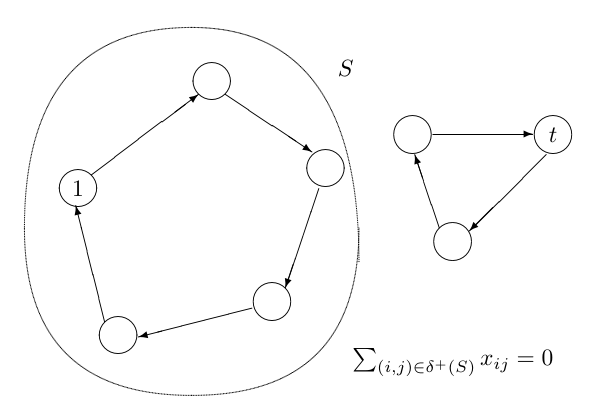
\includegraphics[scale=0.5]{./img/tsp.png}
\end{center}
\caption{Soluzione che viene scartata dal TSP grazie al terzo vincolo del modello}
\label{fig:terzoVincoloTSP}
\end{figure}


\paragraph{Generazione dinamica di vincoli per il TSP}%
\label{par:Generazione dinamica di vincoli per il TSP}
L'idea di base è quella di andare ad introdurre i vincoli iterativamente.
\begin{lstlisting}[language=]
1. Si eliminino tutti i sub-tour elimination constraints e i vincoli di
    interezza della variabili e si risolva il corrispondente problema di 
    assegnamento.
2. Se la soluzione corrente non contiene sotto-cicli allora STOP: soluzione
    ottima.
3. Si individuino uno (o piu') sotto-cicli nella soluzione corrente. 
4. Si aggiungano al modello i vincoli di eliminazione di almeno uno dei 
    sotto-cicli individuati.
5. Si risolva il problema corrente e si torni al passo 2.
\end{lstlisting}
L'approccio di aggiungere iterativamente solo alcuni vincoli è valido in quanto
si osserva che non tutti i vincoli sono necessari per eliminare tutti i sotto-cili.
Il problemi dell'algoritmo riportato sono: il numero elevato di iterazioni e
il fatto che ad ogni iterazione bisogna risolvere un problema di programmazione
lineare intera mista.
Proviamo a migliorare l'approccio usando un algoritmo di ricerca ad albero.

\paragraph{Branch-and-bound per TSP}%
\label{par:Branch-and-bound per TSP}
Migliora le prestazioni rispetto all'algoritmo precedente.
\begin{lstlisting}[language=]
1. Al nodo radice considero il problema completo e, al fine di ottenere un 
    lower bound elimino tutti i vincoli di sotto-ciclo SEC.
2. Risolvo il problema risultante come problema di assegnamento e ottengo un 
    lower bound.
3. Se la soluzione e' intera e non contiene sotto-cicli allora la soluzione e' 
    ottima e non si sviluppano altri nodi.
4. In caso contrario si fa branching generando sotto-problemi le cui soluzioni 
    ammissibili non contengono i sotto-cicli individuati. 
\end{lstlisting}
Non serve che vengano eliminati tutti i sotto-cili individuati nella soluzione del
problema associato ad un nodo, basta eliminare un sotto-ciclo per volta.
Tramite questo processo ripetuto ricorsivamente sui nodi otteniamo un algoritmo
branch-and-bound in grado di risolvere il TSP.
L'algoritmo rimane esponenziale nel caso peggiore.

\paragraph{L'albero di Steiner}%
\label{par:L'albero di Steiner}
Il problema dell'albero di Stainer è un altro esempio di problema di programmazione
lineare intera che sfrutta la generazione dinamica di vincoli.

Abbiamo un grafo diretto $G(V,A)$ in cui vengono definiti i costi $c_{ij}$ associati
ad ogni arco $(i,j) \in A$.
Viene identificato il nodo $r\in V$, chiamato radice e l'insieme dei nodi terminali
$T\subseteq V$.
Il problema consiste nel selezionare un insieme di archi che individua un
albero con radice $r$ e che collega tutti i nodi terminali (al costo minimo).
Definiamo le variabili binarie per la selezione degli archi:
\[
    \forall (i,j) \in A,\quad x_{ij} =
    \begin{cases}
        1 & \text{se } (i,j) \text{ è nell'albero}\\
        0 & \text{altrimenti}
    \end{cases}
\]
il modello è il seguente
\[
    \begin{cases}
        \text{min}\, \sum_{(i,j)\in A} c_{ij} x_{ij}\\
        \sum_{(i,j)\in \delta^-(j)} x_{ij} =
        \begin{cases}
            1 & \text{se } j\in T\\
            0 & \text{se } j = r\\
            \leq 1 & \text{altrimenti}
        \end{cases}\\
        \sum_{(i,j)\in \delta^+(S)} x_{ij} \geq \sum_{(i,t)\in \delta^-(t)} x_{it} & 
        \forall S\subset V,\, r\in S,\quad \forall t \in V\setminus S \\
        x_{ij} \in \left\{ 0,1 \right\} & \forall (i,j) \in A
    \end{cases}
\]
dove
\begin{itemize}
    \item il primo vincolo impone il grado dei nodi;
    \item il secondo vincolo impone che ogni nodo visitato sia raggiunto dalla
        radice, ovvero garantisce la connettività dell'albero.
\end{itemize}
Anche in questo caso il secondo vincolo si porta dietro una famiglia di vincoli
in numero esponenziale visto che il numero di sottoinsiemi $S$ è esponenziale.
Utilizzando la generazione di vincoli dinamica e l'algoritmo Branch-and-bound
possiamo risolvere il problema in tempi ragionevoli.

\begin{figure}[ht!]
\begin{center}
    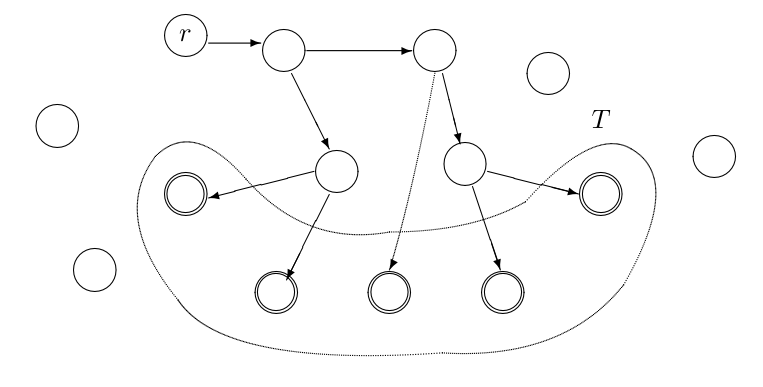
\includegraphics[scale=0.5]{./img/stainerTree.png}
\end{center}
\caption{L'albero di Stainer}
\end{figure}

% Fine documento
\end{document}
